\section{Consensus layer support} \label{sec.consensus}

%\subsection{The interlink pointers data structure}
\label{sec.interlink}

\subsection{The interlink pointers data structure}
In order to construct our protocols, as in \cite{KLS}, we take advantage of a
data structure that will be stored in the header of a block. Observe that in a
blockchain protocol execution it is expected half of the blocks will be of level
$1$, $1/4$ of the blocks will be of level $2$, $1/8$ will be of level $3$ and
$1/2^\mu$ blocks will be of level $\mu$. In expectation, the number of
superblock levels of a chain $\chain$ will be $\Theta(\log(\chain))$ \cite{KLS}.
Figure~\ref{fig.hierarchy} illustrates the blockchain superblocks starting from
level $1$ and going up to level $4$ in case these blocks are distributed exactly
according to expectation. Here, each level contains half the blocks of the level
below.

\begin{figure}
    \caption{The hierarchical blockchain.
    Higher levels have achieved a lower target (higher difficulty) during mining.}
    \centering
    \iftwocolumn
        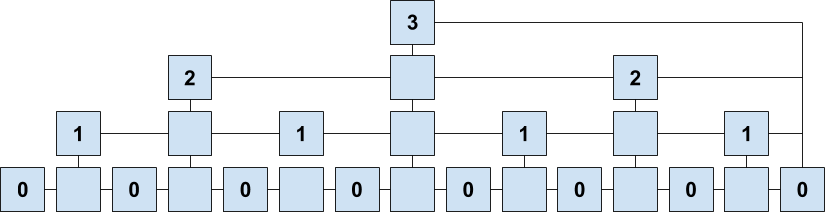
\includegraphics[width=\columnwidth,keepaspectratio]{figures/hierarchical-ledger.png}
    \else
        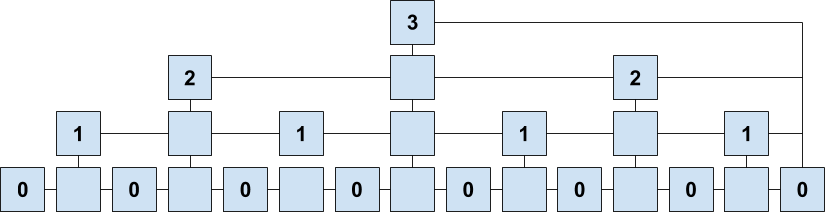
\includegraphics[width=0.7\columnwidth,keepaspectratio]{figures/hierarchical-ledger.png}
    \fi
    \label{fig.hierarchy}
\end{figure}

The \textit{interlink} data structure is proposed to be included in each block,
replacing the existing pointer to the previous block with a list of pointers to
a small number of previous blocks. For each block, this data structure contains
a pointer to the most recent preceding block of every level $\mu$. The algorithm
for this construction is shown in Algorithm~\ref{alg.nipopow-interlink} and is
borrowed from~\cite{KLS}. Genesis is of infinite level and hence a pointer to it
is included in every block at the first available index within the interlink
data structure. The interlink data structure turns the blockchain into a
skiplist-like~\cite{skiplist} data structure.  The number of pointers that need
to be included per block is in expectation $\log(|\chain|)$.

The updateInterlink algorithm accepts a block $B'$, which already has an
interlink data structure defined on it. The function evaluates the
interlink data structure which needs to be included as part of the next block.
It copies the existing interlink data structure and
then modifies its entries from level $0$ to $\textsf{level}(B')$ to
point to the block $B'$.

% \import{./}{algorithms/alg.nipopow-helper.tex}
\import{./}{algorithms/alg.nipopow-interlink.tex}

\subsection{Superchain quality}
In order to argue formally about the security
properties of blockchains that are equipped with the interlink
data structure we will introduce a new concept of {\em superchain quality},
which generalizes the chain quality property from the backbone model~\cite{backbone}.
We stress that the superchain quality is a new contribution in this paper, and is essential for identifying and overcoming the attack on PoPoW.

We first define a notion of ``goodness'' that bounds the deviation
of superblocks of a certain level from their expected mean. Using
this we then define superchain quality.

\begin{definition}[Locally good superchain]
A superchain $\chain'$ of level
$\mu$ with underlying chain $\chain$ is said to be $\mu$-\textnormal{locally-good}
with respect to security parameter $\delta$, written
$\textsf{local-good}_{\delta}(\chain', \chain, \mu)$, if $|\chain'| > (1 -
\delta)2^{-\mu}|\chain|$.
\end{definition}

\begin{definition}[Superchain quality]
The $(\delta, m)$ superquality property $Q^\mu_{scq}$ of a chain $\chain$
pertaining to level $\mu$ with security parameters $\delta \in \mathbb{R}$ and
$m \in \mathbb{N}$ states that for all $m' \geq m$, it holds that
$\textsf{local-good}_{\delta}(C\upchain^\mu[-m':],
C\upchain^\mu[-m':]\downchain, \mu)$. That is, all sufficiently large suffixes
are locally good.
\end{definition}

While superchain quality guarantees that a superchain has a sufficient number
of blocks w.r.t. the level 0 chain, we will also need to be able to compare
it with other superchains. For this reason we introduce multilevel quality.

\begin{definition}[Multilevel quality]
A $\mu$-superchain $\chain'$ is said to have \textit{multilevel quality}, written
$\textnormal{multi-good}_{\delta, k_1}(\chain, \chain', \mu)$ with respect to an
underlying chain $\chain = \chain'\downchain$ with security parameters $k_1,
\delta$ if for all $\mu' < \mu$ it holds that for any $\chain^* \subseteq \chain$,
if $|\chain^*\upchain^{\mu'}| \geq k_1$, then $|\chain^*\upchain^{\mu}| \geq (1 -
\delta)2^{\mu - \mu'}|\chain^*\upchain^{\mu'}|$.
\end{definition}

% For $\delta < 0.5$, multilevel quality implies that
% $|\chain^*\upchain^{\mu}| \geq 1$.

Putting the above together we conclude with the notion of a {\em good} superchain.

\begin{definition}[Good superchain]\label{lem.good}
A $\mu$-superchain $\chain'$ is said to be \textit{good}, written
$\textnormal{good}_{\delta, k_1}(\chain, \chain', \mu)$, with respect to an
underlying chain $\chain = \chain'\downchain$ if it has both superquality and multilevel quality with parameters $(\delta, m)$.
\end{definition}

It is not hard to see that the above good statistical properties are attained
with overwhelming probability by all chains that are generated in optimistic
environments, i.e. if no adversary tries to violate them. This is established in
the following lemmas.

\begin{lemma}[Local goodness]
\label{lem.localgood}
Assume $\chain$ contains only honestly-generated blocks in an optimistic
execution. For all levels $\mu$, for all constant $\delta > 0$, all continuous
subchains $\chain' = \chain[i:j]$ with $|\chain'| \geq m$ are locally good,
$\textsf{local-good}_{\delta}(\chain', \chain, \mu)$, with overwhelming
probability in $m$.
\end{lemma}
\import{./}{proofs/localgood.tex}

\begin{lemma}[Multilevel quality]\label{lem.multilevel}
For all $\mu, 0 < \delta \leq 0.5$, chain $\chain$ containing only
honestly-generated blocks in an optimistic execution has $(\delta, k_1)$
multilevel quality at level $\mu$ with overwhelming probability in $k_1$.
\end{lemma}
% \import{./}{proofs/multilevel.tex}
\begin{proof}
Identical.
\Qed
\end{proof}

\begin{lemma}[Superquality]
\label{lem.superquality}
For all $\mu, \delta > 0$, a chain $\chain$ adopted in an optimistic execution
has $(\delta, m)$-superquality at level $\mu$ with overwhelming probability in
$m$.
\end{lemma}
\import{./}{proofs/superquality.tex}

\begin{lemma}[Optimistic superchain distribution]
\label{lem.superchain-distribution}
For a level $\mu$, and $0 < \delta < 0.5$, a chain
$\chain$ containing only honestly-generated blocks adopted by an honest party in
an execution with random scheduling is $(\delta, m)$-good at level
$\mu$ with overwhelming probability in $m$.
\end{lemma}
\ifonecolumn
\begin{proof}
This is a direct consequence of Lemma~\ref{lem.superquality} and
Lemma~\ref{lem.multilevel}. \Qed
\end{proof}
\fi
